% CREATED BY DAVID FRISK, 2016
\chapter{Methods}
When discussing \textit{accessibility} of a teaching material, in this study, it has been separated into two aspects: \textit{obtainability} and \textit{usability}. Collecting data for these aspects has be done separately and with different methods. The purpose of describing this study's methodology is both to give insight in how data has been collected, as well as describing a methodology one can use when revising their own shareable teaching material.

\section{Obtainability}
Obtainability describes how easy it is for a teacher to obtain a teaching material, and the data for this aspect of accessibility has mainly be acquired through studying literature. Some data connected to obtainability has also been acquired while performing usability testing, partly because these aspect have proven hard to isolate from each other.

\section{Usability}
The main method of collecting data for this study consisted of a process inspired by Adaptive Software Development (ASD). This method involves iterative development with strengths that fit this study, such as being flexible and low risk. This can for example mean that new information
can be easily adopted in future tests and that results can be delivered even if test subjects decide to terminate involvement in this study early. (Sommerville, 2016)\\
ASD is an antecedent to Agile Software Development, paving the way for popular project management methodologies such as Scrum and Kanban. The methodology for this study has no need of being as complex as Scrum or Kanban, one of the main reasons being the relative small size of the development team (i.e. the two authors of this paper), whereas for example the Scrum model is generally used by splitting a larger workforce in teams of 3 to 9. (Schwaber, 2004)\\
As can be seen in Figure \ref{asd} ASD consists of three stages with a feedback loop, enabling developers to perform multiple iterations of improvement based on what they learn from users. This model is similar to the methodology that was developed in this study to collect data on usability of teaching materials. (Highsmith, 2000, p.84)\\

\begin{figure}
\hspace*{-1cm}
\centering
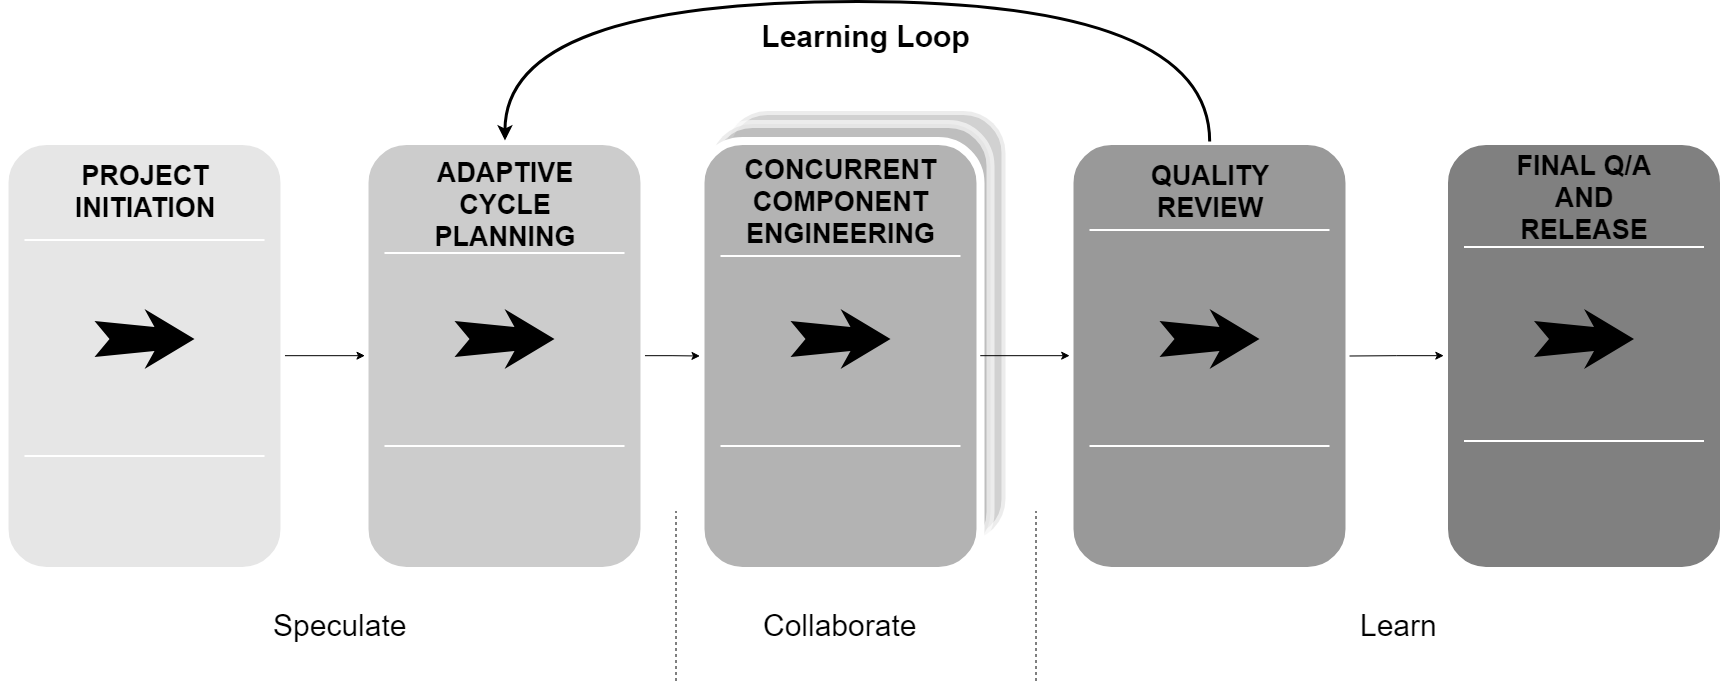
\includegraphics{figure/asd.png}
\caption{A }
\label{asd}
\end{figure}


\subsection{Comparing ASD to the used methodology}
While deciding on the aim of this study, a custom methodology was developed, as this process helped clarify what the study did and did not aim to investigate and how that was expected to play out. That methodology is described in Figure~\ref{workflow}, and then compared to the ASD methodology to indicate similarities and differences.

\begin{sidewaysfigure}
\centering
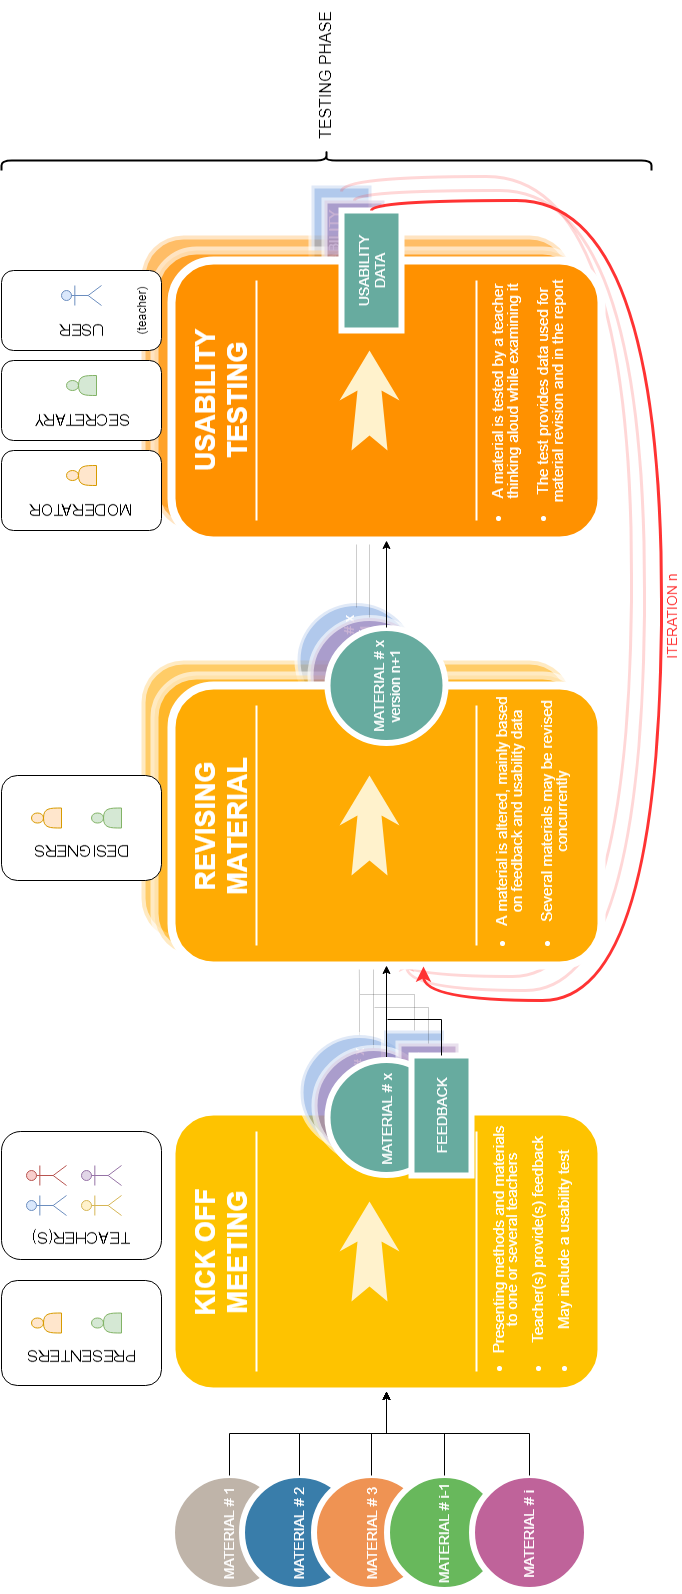
\includegraphics[scale=0.6,angle=-90]{figure/workflow.png}
\vspace*{2cm}
\caption{As with ASD, this custom designed method includes a learning loop and can be used for collecting data on usability
of teaching materials. The method also describes the roles of the different actors, based on the current stage of the testing
phase.}
\label{workflow}
\end{sidewaysfigure}

Comparing the methodology developed for this study with the ASD model, the \textbf{Kick Off Meeting} used to introduce one or more teachers to the study, as well as deciding on a teaching material to work on and a date for the first usability test, is comparable to the \textbf{Project Initiation} of ASD, being prior to the parts contained inside the \textbf{Learning Loop}.\\

What in the ASD methodology is called \textbf{Adaptive Cycle Planning} is the initial step of the \textbf{Revising Material} stage, deciding on how to rework the teaching material based on the data collected from a \textbf{Kick Off Meeting} or previous \textbf{Usability Test}. This is inevitably one of the stages where collected data is summarized and analyzed, even if just as a thought process.\\

The \textbf{Concurrent Component Engineering} part of ASD is practically the same as the \textbf{Revising Material} stage, this is where a coder would revise the code of the program and this is likewise where the product, the teaching material, is being worked on with the intent of improving its
usability.\\

What is called \textbf{Quality Review} in ASD is the \textbf{Usability Testing} part of this study. This is where the teaching material is tested on a teacher and the data needed to improve the usability of the teaching material is collected. The method used to test usability is based on Steve Krug’s script for usability testing websites. Because a teaching material is quite different from a website, oftentimes focusing on interactivity, the script could not be used without some changes. There is however some important aspects of Steve Krug’s script, e.g. not asking leading questions, that is of great importance to the quality of the data and thereby the quality of future revisions of the teaching material. (Krug, 2009)\\

The end goal of ASD is called \textbf{Final QA and Release}. In the case of this thesis, this has been replaced with this final report (not visualized in \ref{workflow}).\\

\subsection{Implementation of methodology}
During the Kick Off Meeting of each teacher involved in the study, the teacher was able to choose what teaching material they wanted to use for their usability testing. A list of sample teaching materials was compiled, consisting of a selection of materials produced at \todo{mention Kleindagarna earlier or describe more here. /H} Kleindagarna. This was done as a compromise between delimiting the study and offering teaching materials that feel relevant to the teachers.\\

When revising material, the decisions of what to revise when is determined from a combination of data from Usability Tests and by studying literature. \todo{The later part of this paragraph brings up something we don't do. /H}There may have been instances where a teacher’s assumptions of how the next revision will look have been unmet. These cases need to be analyzed and mentioned in the final report, as they may lead to interesting discussions. If for example a revision is made following a certain pedagogic template, and the resulting material makes the test subject less inclined to use it on a lesson, new conclusions can possibly be drawn about accessibility of designing teaching materials.


\subsection{Test subject anonymity}
There are several ways of presenting the personal details of test subjects in scientific studies. In this study some personal details have been disclosed and some have been held anonymous. What is disclosed and examples of what is held anonymous are listed below.

\subsubsection*{Disclosed information}
    \begin{itemize} %Disclosed information
    \item Age – rounded to nearest 5 years.
    \item Current status – if the test subject is currently working as a teacher and if so on what stage of education, or if they are e.g. studying to become a teacher.
    \item Years in teaching – nearest year if under 10 years, can otherwise be rounded to nearest 5 years. No regard to the age of students taught. No regard to full-time or part-time employment.
    \item Subjects – what school subjects is the test subject certified to teach or studying to teach?
\end{itemize}

\subsubsection*{Anonymous information}
\begin{itemize} %Anonymous information
    \item Sex/Gender – the risk of a reader finding false correlations from the data is assumed to be greater if the test subject’s sex and/or gender is disclosed.
    \item Name – the name of the test subjects will not be disclosed, and because the sex/gender will not either, the label of the test subjects will also be as gender free as possible.
    \item Name of school – with this information, it would be too easy to identify the test subject.
    \item Place of school – all subjects studied will live and work in close proximity to Gothenburg, Sweden, as it has been decided to delimit the tests to personal meetings.
\end{itemize}